\section{Teoria Dei Codici}
    \subsection{Introduzione}
        Ci concentriamo adesso sul trattamento dell'informazione per poterla trasmettere.
        I messaggi che trasmettiamo possono essere codificati per vari motivi:
        \begin{itemize}
            \item {
                    Compressione:$\begin{cases}
                        \text{Lossy: con perdita dell'informazione} \nonumber\\
                        \text{Lossless: minima perdita dell'informazione} \nonumber
                    \end{cases}$\\
                    Comprimere l'informazione in elimenando ridondanza e salvando spazio di memoria e banda.
                    
                }
            \item {
                    Crittografia: per nascondere il messaggio ad utenti in ascolto sul canale che non siano il destinatario.
            }
            \item {
                    Rivelazione o correzione di errore: vieen aggiunta ridondanza ad hoc per aumentare l'affidabilitá del messaggio trasmesso. 
                    Si utilizzano \href{https://en.wikipedia.org/wiki/Checksum}{checksum} o \href{https://en.wikipedia.org/wiki/Reed-Solomon_error_correction}{Reed-Solomon(RS)}
            }
        \end{itemize}

        \paragraph{Canale Gaussiano}
            Il canale Gaussiano puó essere modellato come \href{https://en.wikipedia.org/wiki/Binary_symmetric_channel}{Binary Symmetric Channel (BSC)} con probabilitá di errore $p$. 
            Assumiamo gli errori tra loro indipendenti ($p_{(a,b)} = p_{(a)}\dotproduct p_{(b)}$):
        \begin{figure}[H]
            \centering
            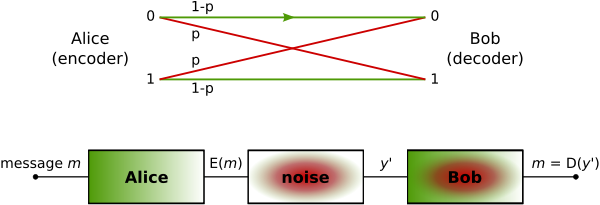
\includegraphics[width = 12cm]{media/600px-Binary_symmetric_channel_(en).svg.png}
            \label{BSC system}
            \caption{Sistema di trasmissione BSC}
        \end{figure}
        \begin{gather}
            E_{(x)}: \text{Funzione di codifica} \nonumber \\
            D_{(x)}: \text{Funzione di decodifica} \nonumber \\
            E_{(m)}: \text{Bit dell'informazione codificati} \nonumber \\
            y^\prime: E_{(m)}+ e \rightarrow \text{Informazioni con errore del canale} \nonumber \\
            m = D_{(y^\prime)}: \text{Informazione decodificata} \nonumber 
        \end{gather}
        Il canale é chiamato simmetrico perché ho la stessa probabilitá errore sulla trasmissione di uno dei due bit. 
        \paragraph{Tassonomia dei codici}
            \begin{itemize}
                \item {Codici lineari
                        \begin{itemize}
                            \item {
                                Codici a blocco
                                }
                            \item{
                                Codici convoluzionali
                            } 
                        \end{itemize}
                    }
                \item {
                    Definizione di un codice a blocco: 
                    \begin{figure}[H]
                        \centering
                        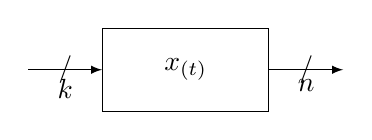
\begin{tikzpicture}[
                            node distance=2cm,
                            >=latex
                            ]

                            \node [coordinate] (input) {};
                            \node [draw, rectangle,right of = input, minimum height=3em, minimum width=6em] (block) {$x_{(t)}$};
                            \node [coordinate, right of = block] (output) {};
                            
                            \draw[draw,->] (input) -- node[midway]{$/$} node[below]{$k$} (block);
                            \draw[->] (block) -- node[midway]{$/$} node[below]{$n$} (output);
                        \end{tikzpicture}    
                    \label{Def codice a blocco}
                    \end{figure}
                }
                \item 
                \item 
            \end{itemize}

        \subsubsection{Esempio codici a blocco: codici a ripetizione}
            
        \subsubsection{Esempio codici a blocco: codici a controllo di paritá}

        \subsubsection{Esempio codici a blocco: codice ISBN}
    \subsection{Codici a blocco}
        \subsubsection{Introduzione ai codici lineari}
            {Definizione di campo}
        \subsubsection{Campi di Galois}

        \subsubsection{Codici a blocco lineari su $GF(2)$}
        n>k perché nei codici io metto cose in piú che magari non mi servono amplio le cose.\\


        \subsubsection{Propietá dei codici a blocco lineari}
            \begin{itemize}
                \item {1}
                \item {2}
                \item {3}
                \item {4}
                \item {5}
            \end{itemize}
        \subsubsection{Distanza di Hamming}
            

            Peso di hamming.
            distanza minima di un codice

        \subsubsection{Codici a blocco in forma sistematica}
            \begin{itemize}
                \item {1 matrici che generano codici equivalenti }
                \item {2 qualsiasi codice lineare a blocchi é equivalente a un codice in forma sistematica}
                \item {3}
                \item {4}
                \item {5}
                \item {6 codici equivalenti}
            \end{itemize}

        se non é una parola di codice la matrice H ci informa con un vaolre 1 nel prodottod